% Licensed to the Apache Software Foundation (ASF) under one or more
% contributor license agreements. See the NOTICE file distributed with
% this work for additional information regarding copyright ownership.
% The ASF licenses this file to You under the Apache License, Version 2.0
% (the ``License''); you may not use this file except in compliance with
% the License. You may obtain a copy of the License at
%
% http://www.apache.org/licenses/LICENSE-2.0
%
% Unless required by applicable law or agreed to in writing, software
% distributed under the License is distributed on an ``AS IS'' BASIS,
% WITHOUT WARRANTIES OR CONDITIONS OF ANY KIND, either express or implied.
% See the License for the specific language governing permissions and
% limitations under the License.

\begin{changemargin}{1.5in}{0in}

\section{Overview}

The MetaCarta GTS appliance indexes documents and allows users to
search these documents based on both keywords and geographic
references. The MetaCarta FileNet Connector allows system
administrators to configure connections and define jobs to ingest
documents from IBM\circler\ FileNet\circler\ repositories.

This document specifies the means for connecting to FileNet
repositories, indexing files from these repositories, and maintaining
connections to these repositories.

\subsection{Assumptions}

This document assumes you have a basic level of familiarity with GTS
appliance administration. This document also assumes that you have a
basic understanding of the repositories to which you are trying to
connect. If you need more information about the MetaCarta GTS
appliance, please read the \documentref{MetaCarta GTS Administrator's
Guide} stored on the appliance at
\dirpath{/usr/share/doc/metacarta/AdminGuide.pdf}.

For more information about FileNet, contact your FileNet administrator
or view IBM's documentation at
\url{http://www-01.ibm.com/software/data/content-}\linebreak\url{management/}.

Throughout this document, we assume that your appliance is named \\
\url{metacarta.example.com}.

\section{Installation}

The FileNet Connector must be used with the MetaCarta Connector
Framework, described in the \documentref{Metacarta Connector
Guide}. If you already have the Connector Framework installed, you can
install the FileNet Connector.  The Filenet Connector is
available as a field-test addon ISO file from from Metacarta. Use the
following steps to install the Sharepoint Connector to your appliance:

\begin{enumerate}

\item Confirm that the system is running correctly using
\command{check\_system\_health}.

\item Copy the disc image and md5sum supplied by MetaCarta to the
\dirpath{/isos} directory on your appliance. Rename the ISO file to
\dirpath{addon-fln-conn.iso} when you copy it to your appliance.

\item Check the md5sum of the ISO file using the \command{md5sum} command.

\item Install the iso using the following command:

\command{upgrade\_control install /isos/addon-fln-conn.iso}

The appliance will reboot once the installation is complete.

\item Upgrade your license file, if necessary, as described in
\documentref{MetaCarta Appliance Administrator's Guide}. You may need
to contact MetaCarta Customer Service to obtain the appropriate
license file. (Please see page \pageref{SupportContact} for contact
information.)
 
\end{enumerate}

\section{Configuration}

\subsection{Access to the Connector}

The administrator to the FileNet Connector % Licensed to the Apache Software Foundation (ASF) under one or more
% contributor license agreements. See the NOTICE file distributed with
% this work for additional information regarding copyright ownership.
% The ASF licenses this file to You under the Apache License, Version 2.0
% (the ``License''); you may not use this file except in compliance with
% the License. You may obtain a copy of the License at
%
% http://www.apache.org/licenses/LICENSE-2.0
%
% Unless required by applicable law or agreed to in writing, software
% distributed under the License is distributed on an ``AS IS'' BASIS,
% WITHOUT WARRANTIES OR CONDITIONS OF ANY KIND, either express or implied.
% See the License for the specific language governing permissions and
% limitations under the License.

must have
access to the web interface at
\url{http://metacarta.example.com/crawler/}. In the default appliance
security setup, you must have a Basic Authentication account
configured for access to the Connector web interface at
\url{http://metacarta.example.com/crawler/}.  If you are not an appliance
administrator, please ask the appliance administrator to give you such
an account.

An appliance administrator can create an account with access to the
ingestion interface (in this case, username {\tt fred} and password
{\tt ginger}) by running the following command on the appliance:

\begin{console}
metacarta:\~{}\$ basic\_auth\_control add ingest\_users fred:ginger 
\end{console}

Depending on how you have configured authentication using the
\command{auth\_control} tool, you may need to make changes other than
adding yourself to the ingest\_users group. For more information on
security configuration and \command{auth\_control}, see the Security
Administration section of the \documentref{MetaCarta Appliance
Administrator's Guide}.


\section{Collecting Documents From FileNet Repositories} % Retitle this, yo.

The Connector Framework manages retrieving documents from different
feeds and repositories through \emph{jobs}. Jobs can be scheduled to
run regularly; each job connects to a single repository using a
particular set of credentials. Each job is tied to a \emph{repository
connection}. Repository connections contain information allowing the
connector framework to connect to a given repository. A repository
connection may be tied to an \emph{authority connection}, which
manages document security. While using the FileNet Connector to
connect to a FileNet repository, no authority connection is needed;
you can simply create a repository connection.


\subsection{Creating Repository Connections}

In order to create jobs to ingest documents, you need to create a
repository connection. To do so, click ``List Repository
Connections'' on the sidebar menu. Then, when presented with the list
of repository connections, click ``Add a new connection.'' You will
see the following two tabs:

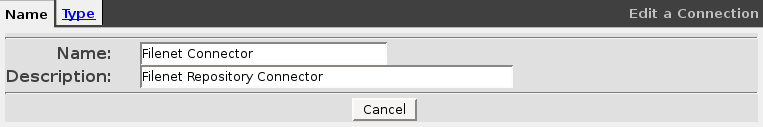
\includegraphics[width=300pt]{fln-edit-repository-tab1}

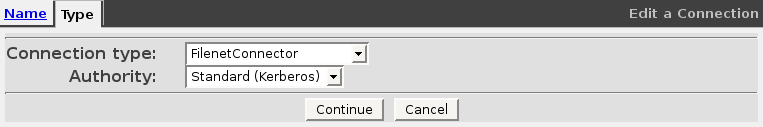
\includegraphics[width=300pt]{fln-edit-repository-tab2}



% Licensed to the Apache Software Foundation (ASF) under one or more
% contributor license agreements. See the NOTICE file distributed with
% this work for additional information regarding copyright ownership.
% The ASF licenses this file to You under the Apache License, Version 2.0
% (the ``License''); you may not use this file except in compliance with
% the License. You may obtain a copy of the License at
%
% http://www.apache.org/licenses/LICENSE-2.0
%
% Unless required by applicable law or agreed to in writing, software
% distributed under the License is distributed on an ``AS IS'' BASIS,
% WITHOUT WARRANTIES OR CONDITIONS OF ANY KIND, either express or implied.
% See the License for the specific language governing permissions and
% limitations under the License.

\begin{picture}(1,1)
  \put(-100,15){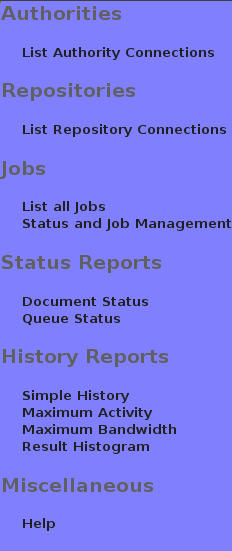
\includegraphics[width=80pt]{crawler-sidebar}}
\end{picture}




Now you must provide a name, description, and connector type for your
new repository connection. The name should be unique, as you will use
it to select this connection later when defining jobs. The description
should explain the repository connection to you or another
administrator.  The connector type is the type of repository from
which you will get documents, in this case a FilenetConnector. The
authority type is the type of authority from which you will get
authorization information. The FileNet Connector does not use an
administrator-created authority; you should simply select ``Standard
(Kerberos)'' here.

Once you have filled in those tabs, click Continue to be taken to the
repository-specific options.

% Licensed to the Apache Software Foundation (ASF) under one or more
% contributor license agreements. See the NOTICE file distributed with
% this work for additional information regarding copyright ownership.
% The ASF licenses this file to You under the Apache License, Version 2.0
% (the ``License''); you may not use this file except in compliance with
% the License. You may obtain a copy of the License at
%
% http://www.apache.org/licenses/LICENSE-2.0
%
% Unless required by applicable law or agreed to in writing, software
% distributed under the License is distributed on an ``AS IS'' BASIS,
% WITHOUT WARRANTIES OR CONDITIONS OF ANY KIND, either express or implied.
% See the License for the specific language governing permissions and
% limitations under the License.

\subsubsection{Configuring a FileNet Connector}

You must fill in the following tabs if you are configuring a
FileNet Connector:

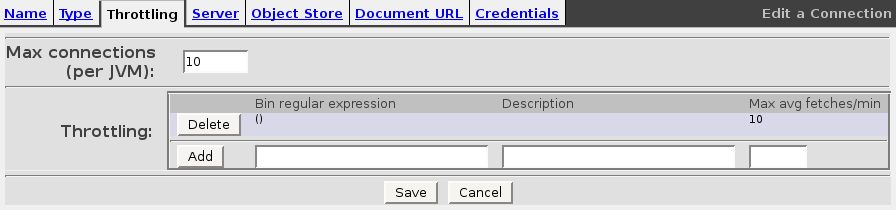
\includegraphics[width=300pt]{fln-edit-repository-tab3}

\begin{itemize}

\item \textbf{Max connections (per JVM):} Here you can set the maximum
number of connections to your repository.  \ifCombinedConnectorGuide
The maximum number of connections per JVM is important for three
reasons; licensing, appliance resources, and the possiblity of
overwhelming the ingestion interface. For a more complete explanation,
see the Max Connections item on page \pageref{maxrepocon}.\fi

\ifJDBCGuide
The maximum number of connections per JVM is important for several
reasons.  First, the number of connections may impact licensing and
available resources on your FileNet server.

Second, the number of connections may impact the resources available
on the appliance. If the connector framework is slowing down your
appliance, lowering this number should help.

Third, only ten document streams can be processed by the appliance
at one time.  If you are also using other repository connectors or
the \command{ingest} command on the appliance, you should reduce this
number to prevent contention for the Ingestion interface. The FileNet 
Connector will never overwhelm the interface on its own, but when other
applications are also using the ingestion interface, it may be best to
set the number of repository connections to five or even fewer.
\fi


\item \textbf{Throttling:} Here you can set a maximum document fetch
rate for the repository connection.  The maximum fetch rate allows you
to set three things: Expression, description, and fetches per minute.

In the FileNet Connector, the expression field can be used to create
throttle groups based on server name. Each FileNet Repository
Connection connects to only one server; use the blank match expression
\texttt{()} to match the server. Ask your FileNet administrator for an
appropriate limit on the number of fetches per minute. Enter the
information, and click Add.

\end{itemize}

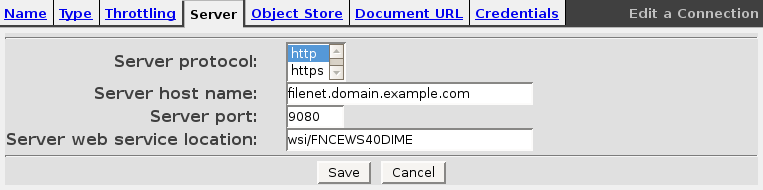
\includegraphics[width=300pt]{fln-edit-repository-tab4}

To fill out this tab, you will need information about the FileNet
service with which you wish to connect. You should ask your FileNet
administrator for this information.

\begin{itemize}

\item \textbf{Server protocol:} Select ``http'' or ``https'' using the drop down box. 

\item \textbf{Server host name:} The host name (including domain information) of your FileNet server.

\item \textbf{Server port:} The port to use to connect to the server. You should ask your FileNet administrator for the correct port.

\item \textbf{Server web service location:} The location of the FileNet web service on the server specified above.

\end{itemize}

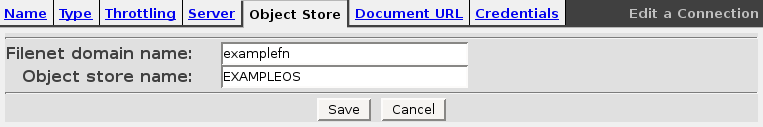
\includegraphics[width=300pt]{fln-edit-repository-tab5}

On this tab you will need to enter the FileNet domain name and object
store name. You will need to ask your FileNet administrator for this
information.

\begin{itemize}

\item \textbf{Filenet domain name:} The FileNet domain for the FileNet services. This is \textbf{not} the same as the Active Directory domain that your FileNet server is joined to.

\item \textbf{Object store name:} The name of the object store that you wish to crawl.

\end{itemize}

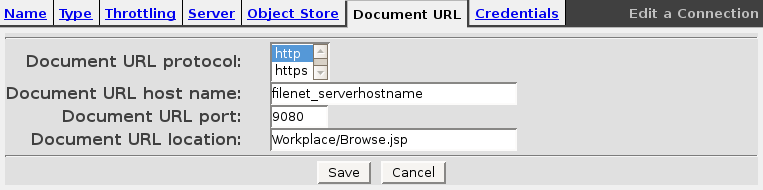
\includegraphics[width=300pt]{fln-edit-repository-tab6}

The information that you provide on this tab will be used to create
document URLs for the crawled documents. You should ask your FileNet
administrator for the information for your FileNet Access Engine.

\begin{itemize}

\item \textbf{Document URL protocol:} Select ``http'' or ``https'' using the drop down box. 

\item \textbf{Document URL host name:} The hostname of the Access Engine server.

\item \textbf{Document URL port:} The port to use to connect to the FileNet Access Engine server.

\item \textbf{Document URL location:} The location of the FileNet Access Engine service.

\end{itemize}

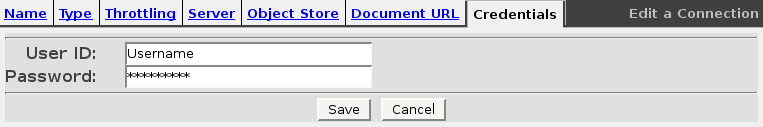
\includegraphics[width=300pt]{fln-edit-repository-tab7}

\item \textbf{User name:} This should be the user name used by your MetaCarta appliance, typically an Active Domain user name in the format \texttt{domain$\backslash$username}.

\item \textbf{Password:} The password corresponding to the user name given.



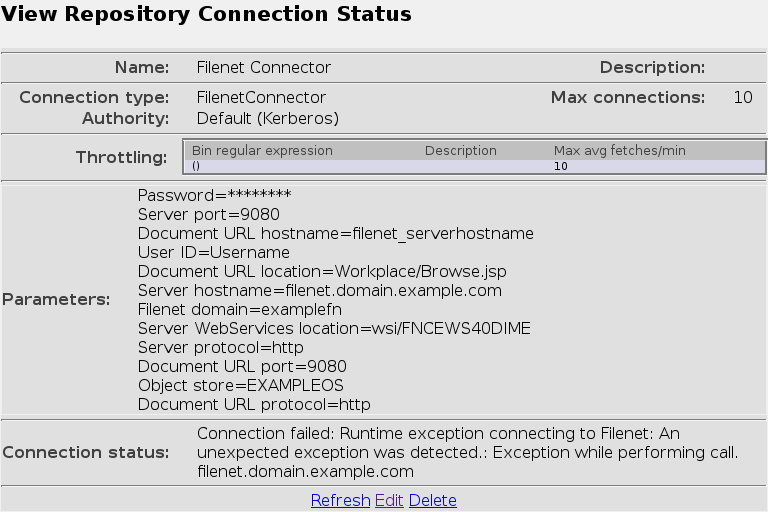
\includegraphics[width=300pt]{fln-view-repo-conn-status}

In this example (which does not contain accurate information for any
FileNet Connector), the Connection Status is ``Connection failed.''
If connetion has failed, the status message may contain information about
the failure.  If you see an error message, the FileNet server might be
down, or you might have incorrectly entered data into one of the fields,
If so, you should click ``Edit'' to fix the data. If you have entered
everything as you intended, please inform your database administrator;
you may not have been given the correct information.


\subsection{Creating and Running Jobs}

To run a job, click ``Status and Job Management'' on the sidebar menu.
You can run or edit existing jobs from this menu.

To create a new job, click ``List All Jobs'' on the sidebar menu. Then, when
presented with the list of current jobs, click ``Add a new job.'' You
will be presented with two tabs, in which you must fill in the following
information:

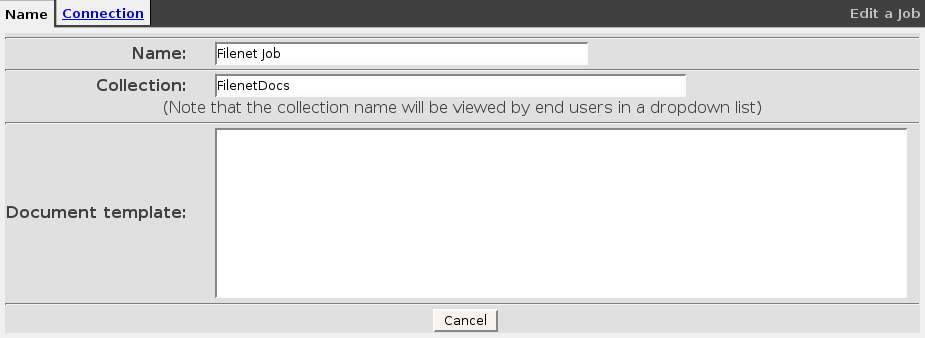
\includegraphics[width=300pt]{fln-edit-job-tab1}

\begin{itemize}

\item \textbf{Name:} The name of the job. You will use this to identify
the job later.

\item \textbf{Collection:} The collection name metadata for all
documents in this job. End users can use this name to select the set
of documents in this job. For more information on collection name
metadata, please see the \documentref{MetaCarta GTS Administrator's
Guide}.

\item \textbf{Document template:} % Licensed to the Apache Software Foundation (ASF) under one or more
% contributor license agreements. See the NOTICE file distributed with
% this work for additional information regarding copyright ownership.
% The ASF licenses this file to You under the Apache License, Version 2.0
% (the ``License''); you may not use this file except in compliance with
% the License. You may obtain a copy of the License at
%
% http://www.apache.org/licenses/LICENSE-2.0
%
% Unless required by applicable law or agreed to in writing, software
% distributed under the License is distributed on an ``AS IS'' BASIS,
% WITHOUT WARRANTIES OR CONDITIONS OF ANY KIND, either express or implied.
% See the License for the specific language governing permissions and
% limitations under the License.

You may also input a document template. A document template, written
in XML, limits the parts of the document that are indexed.  Simply
input the XML in the text entry field.  For information on how to
construct a document template, please see the \documentref{MetaCarta
Document Templates Integrator's Guide}.


\end{itemize}

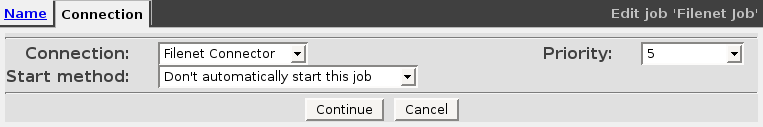
\includegraphics[width=300pt]{fln-edit-job-tab2}

\begin{itemize}

\item \textbf{Connection:} The name of the repository connection you
wish to use for this job. You select this from the list of repository
connections you have already made. You may have more than one job use
the same repository connection, but if you have two jobs crawl the same
documents, the documents will have the metadata and collection name
associated with whatever job crawled the document most recently. This
will cause unpredictable results when searching those collections,
searching for those documents, or trying to delete those collections.
We recommend never crawling the same document in two different jobs.

\item \textbf{Start method:} Whether you want to start this job the next
time jobs are scheduled to run (``Start when schedule window starts''),
immediately after you finish defining it (``Start even inside a schedule
window''), or not at all (``Don't automatically start this job'').

\item \textbf{Priority:} From 1 (highest) to 10 (lowest), the priority
this crawl should have if it must compete for resources with other
crawls on the appliance. You should not need to change this unless you
are running more than one crawl at the same time; if you are, assign a
higher priority to the crawls whose documents you want to be processed
preferentially before documents from other jobs.

\end{itemize}

After filling in those options, click ``Continue'' and you will be
presented with two additional repository-specific tabs.

% Licensed to the Apache Software Foundation (ASF) under one or more
% contributor license agreements. See the NOTICE file distributed with
% this work for additional information regarding copyright ownership.
% The ASF licenses this file to You under the Apache License, Version 2.0
% (the ``License''); you may not use this file except in compliance with
% the License. You may obtain a copy of the License at
%
% http://www.apache.org/licenses/LICENSE-2.0
%
% Unless required by applicable law or agreed to in writing, software
% distributed under the License is distributed on an ``AS IS'' BASIS,
% WITHOUT WARRANTIES OR CONDITIONS OF ANY KIND, either express or implied.
% See the License for the specific language governing permissions and
% limitations under the License.

\subsubsection{FileNet Job Options}

You must fill in four more tabs to configure a FileNet job.

\bigimage{fln-edit-job-tab3}

\ifJDBCGuide
% Licensed to the Apache Software Foundation (ASF) under one or more
% contributor license agreements. See the NOTICE file distributed with
% this work for additional information regarding copyright ownership.
% The ASF licenses this file to You under the Apache License, Version 2.0
% (the ``License''); you may not use this file except in compliance with
% the License. You may obtain a copy of the License at
%
% http://www.apache.org/licenses/LICENSE-2.0
%
% Unless required by applicable law or agreed to in writing, software
% distributed under the License is distributed on an ``AS IS'' BASIS,
% WITHOUT WARRANTIES OR CONDITIONS OF ANY KIND, either express or implied.
% See the License for the specific language governing permissions and
% limitations under the License.

\begin{itemize}
\label{scheduling}

\item \textbf{Schedule type:} Whether you want to scan every document
once or dynamically recrawl content in your repository. 

When scanning every document once, the crawler marks all documents that
have been previously crawled in this job as potentially to be deleted,
adds all seed documents to its queue and marks them as pending, processes
pending documents, marking them completed as they are ingested, and then
deleted all of the documents that were not recrawled. A document might
not be recrawled because it no longer exists, or the job specification
might have been changed to no longer include the document.

When dynamically recrawling documents, the crawler does not start by
marking all documents as potentially deletable; instead, it begins with
all of the seed documents, and continues adding to its list, periodically
re-adding the initial seed documents. If a document is removed from the
source, it will expire in the expiration interval (see below).

\item \textbf{Expiration Interval (if continuous):} The length of the
interval (in minutes) that the appliance will retain a document
crawled by this job after the document no longer appears in the
repository. After this interval, the missing document will be removed
from the appliance's index and archive. Leave the expiration interval
blank to keep missing documents indexed in GTS.

\item \textbf{Recrawl interval:} If you are dynamically recrawling
documents, how long, in minutes, the crawler should wait before
crawling documents a second time.

\item \textbf{Reseed interval:} If you are dynamically recrawling
documents, how long, in minutes, the crawler should wait before
looking for new documents to crawl. \ifMeridioGuide This connector
identifies all documents for ingestion through seeding; if the reseed
interval is infinite, the job will not ingest documents placed in the
repository during run time. (The job automatically reseeds whenever it
is started.) The default interval of 60 minutes is an appropriate
reseed rate. \fi \ifFilenetGuide This connector identifies documents
for ingestion during seeding. If you change the document inclusion
criteria, reseeding is required to identify new documents. Similarly,
documents placed in the repository while the job is running will not
be identified until the crawl is reseeded.  (The job automatically
reseeds whenever it is started.) The default interval of 60 minutes is
an appropriate reseed rate. \fi

\item \textbf{Scheduled time:} Allows you to define a time you wish
the job to run using a series of selection boxes. The first box refers
to the day of the week you wish the job to run, with an option to have
the job run any day of the week. The second box allows you to select
the start hour, with an option to start the job at any hour. The third
box allows you to specify which minute after the hour that you wish
the job to start. The fourth box allows you to specify what months of
the year you wish the job to run, with an option for the job to run
any month. The last box allows you to specify the day of the month you
wish the job to start, including any day of month.


You can scroll through each of the five boxes in this setting using
the arrow keys on your keyboard or by using the scroll bar on the
right side of the box.  If you want to select more than one value,
hold down control as you scroll and click the values that you want to
select. This allows you to define multiple windows with the same
length, for example by selecting Monday, Wednesday, and Friday at the
same time.

\item \textbf{Maximum run time:} The longest you will allow the job to
run, in minutes. For example, if you want to start a job at 2 AM but
force it to stop at 8 AM so that users have access to the repository,
you should set this value to 360 minutes. If the job is not complete by the
end time, documents that have already been found will be indexed, and
the rest of the crawl will continue at the beginning of the next
schedule interval. 

When you have defined the scheduled time and assigned a maximum run
time, click on the ``Add Scheduled Time'' button. A new schedule box
will appear below the scheduled time, allowing you to create
additional scheduled run times.

Here is a sample schedule for a job that will run every
Monday from 2 am to 6 am:

\begin{changemargin}{-.3in}{0in} 
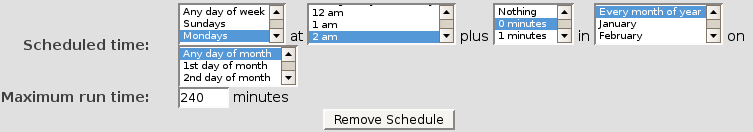
\includegraphics[width=300pt]{sample-schedule}
\end{changemargin}

If you do not have at least one scheduled time, the job will
only run when run manually (see page \pageref{ManageJobs}), and will
not automatically update the index on the appliance based on changes
to the repository.

You can remove a scheduled time by clicking the ``Remove Schedule''
button.

\end{itemize}

\fi

\ifCombinedConnectorGuide
This tab presents scheduling options. Here you can generate one or
more scheduled run times for the job. For a complete description of
the scheduling options, see the description starting on page
\pageref{scheduling}.
\fi

\bigimage{fln-edit-job-tab4}

Here on the Document Classes tab, you can configure which document
classes are ingested by this job, impose match conditions on documents
for ingestion based on metadata, and select which metadata will be
ingested with these documents. Each document class has its own section
on the tab with the following configuration options.

\begin{itemize}

\item \textbf{Include?}
Check this box to include this document class in your crawl.

\item \textbf{Document Criteria:}
Here you can place match conditions based on metadata that will limit
which documents are ingested. By default, all documents of the given
class are ingested if the ``Include'' box is checked.

Match expressions are created by selecting a metadata attribute, a
match type, and entering a match string. First, select any of the
metadata attributed to the document class to use in the match
expresssion from the selection box on the left. Using the drop down
box, select the desired match type. An ``Equals'' expression will
include all documents whose metadata attribute is equal to the match
string you specify in the text box on the right. A ``Not equals''
expression will include all documents whose metadata attribute is not
equal to the match string. A ``'Like' (with \% wildcards)'' expression
includes all documents whose metadata attribute is matched by a
wildcard match string. The \% wildcard matches zero or more
characters. You can use it to create match expressions such as
``\%Test\%'', which will match any string containing Test, or
``Test\%'', which will match any string beginning with Test.

Once you select a metadata attribute, a match type, and enter a match
string, click the ``Add'' button to the left of the expression. The
match expressions will appear above the selection area. You can
continue to add more match expressions. To delete a match expression,
simply click the delete box that appears to the left of each
expression.

\note{The ``Ingest?'' box must be selected for match expressions to apply.}

\item \textbf{Ingest all metadata fields?}
If you wish to ingest all metadata fields, simply check this box.

\item \textbf{Metadata fields:}
Use this box to select metadata fields for ingestion
individually. Hold the ``Shift'' key while clicking to select a
range. Hold the ``Ctrl'' key while clicking to allow multiple
selections. You can combine these effects.


\end{itemize}

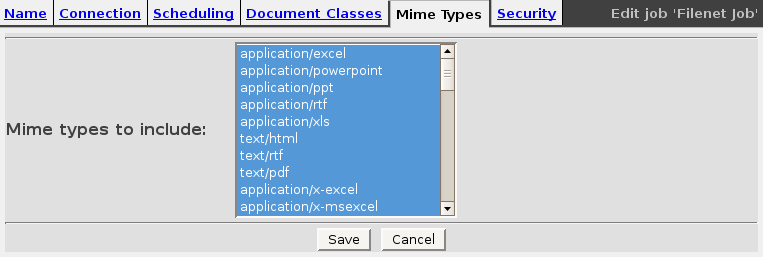
\includegraphics[width=300pt]{fln-edit-job-tab5}

\begin{itemize}

\item \textbf{Mime types to include:}
Here you can select which mime types to include in your searches from
a list of types generated by the appliance. Initially, all mime types
are selected. You can select a single type by clicking on it, which
clears all other selections. To keep previous selections, hold the
``Ctrl'' key while clicking. Holding the ``Shift'' key while clicking
allows you to select ranges. You can combine these effects to select
multiple ranges.


\end{itemize}

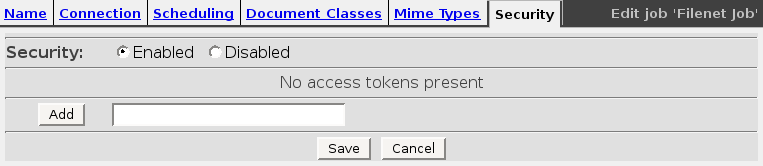
\includegraphics[width=300pt]{fln-edit-job-tab6}

\begin{itemize}



\item \textbf{Security:} Select ``Enabled'' to use Active Directory
permissions with the ingested documents. You can configure custom
permissions using the ``Access Tokens'' tools, or accept the ACLs
as given in the FileNet repository. Select ``Disabled'' to allow all
document search users to access to the files ingested by this job.

\note{If you wish to enforce security, your appliance should be joined
to an appropriate Active Directory domain.}

\item \textbf{Access Tokens:} This field allows you to create custom ACLs
for the files ingested by this job. Enter the SID of a user or group
that you wish to add to the custom ACLs for documents from this job,
then click the ``Add'' button. You can continue to add more SIDs. These
SIDs will appear in a list. Click the ``Delete'' button next to any SID
to remove it from the list.

\end{itemize}


After entering this information, you will be taken to the status page
for this job:

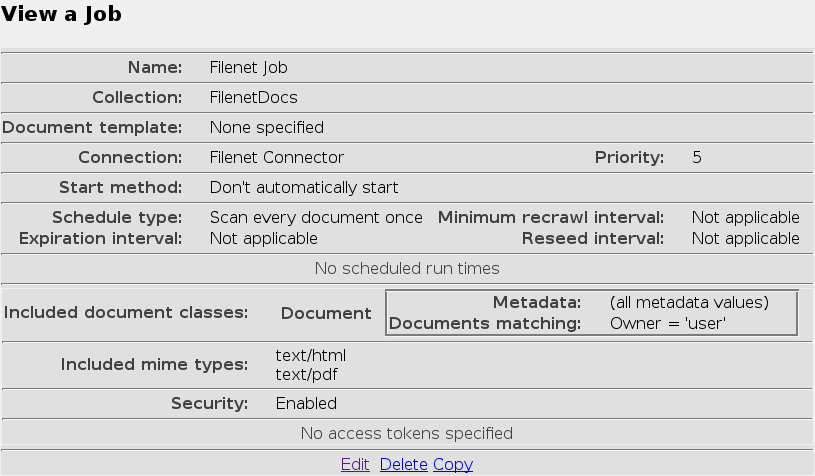
\includegraphics[width=300pt]{fln-view-job-status}




\subsection{\label{ManageJobs}Status and Job Management}

You can then look at the status of your job by clicking ``Status and 
Job Management'' on the sidebar. You will see a list of one or more jobs
much like this one:

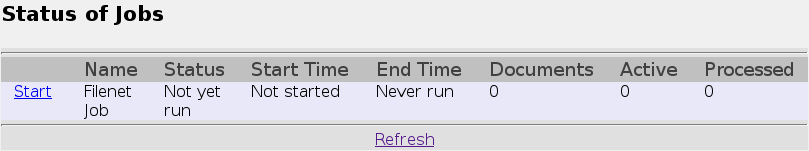
\includegraphics[width=300pt]{fln-jobs-list}

You can start any crawl you like immediately from this interface by
clicking ``Start'' next to the name of the crawl. This interface also
allows you to see how many documents have been crawled; this information
may help you structure and plan future crawls.

\note{Refresh this page by clicking the ``Refresh'' link at the bottom
of the page, not by clicking your browser's reload button.}

\section{Reports}

The Connector interface can generate two types of status reports, on
current crawl status, and four types of history reports, on past crawl
history.

\subsection{Status Reports}

The two types of status report are:

\begin{itemize}

\item Document Status, which lets you find information on individual
documents currently part of a job.

\item Queue Status, which lets you aggregate information about groups
of documents currently part of a job.

\end{itemize}

\subsubsection{Document Status}

This report was generated by selecting ``Filenet Connector,''
selecting the document state ``Documents processed at least once,''
selecting all possible document statuses, clicking continue, selecting
``Filenet Job,'' and clicking Go.

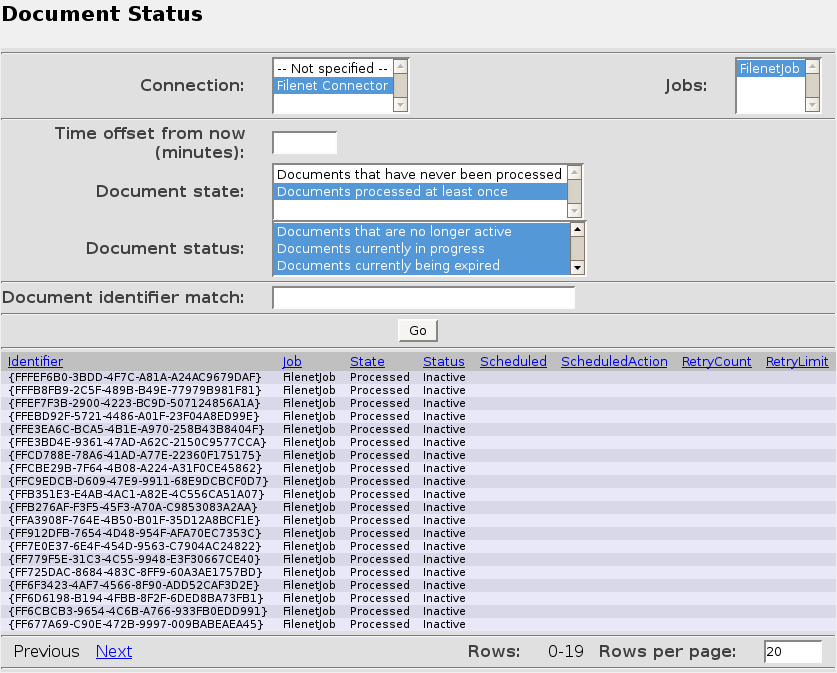
\includegraphics[width=300pt]{fln-document-report}

\begin{itemize}

\item \textbf{Connection:} The repository connection from which to 
generate a report. You must select the repository connection and click
Continue to see all repository-specific options.

\item \textbf{Time offset from now:} Defaults to zero. Allows you to
see estimates of future status or, with negative numbers, a record of
past status.

\item \textbf{Document state:} Allows you to select documents that
have not yet been processed or documents that have been processed
at least once.

\item \textbf{Document status:} Allows you to choose one or more 
statuses of document to report on. The statuses you can choose are:

\begin{itemize}

\item Documents that are no longer active

\item Documents currently in progress

\item Documents currently being expired

\item Documents currently being deleted

\item Documents currently available for processing

\item Documents currently available for expiration

\item Documents not yet processable

\item Documents not yet expirable

\end{itemize}

\item \textbf{Document identifier match:} \label{docid} A regular
expression allowing you to see only documents with matching
identifiers. Here, document identifiers are FileNet version
GUIDs. These GUIDs are 32 character hexidecimal numbers enclosed in
braces. The characters are dash-separated into groupings of eight,
four, four, four, and twelve. For example,
\texttt{\{A19D1286-5CF5-C109-5D49-}\linebreak\texttt{677F576902BA\}}
would be a valid document identifier.

\item \textbf{Jobs:} The job or jobs for which you want to generate
a report.

\end{itemize}

You can sort this report by any of the returned fields; to do so,
click the field names.

\subsubsection{Queue Status}

This report was generated by selecting ``Filenet
Connector,'' selecting both document states, selecting all possible
document statuses, clicking continue, selecting ``Filenet Job,''
and clicking Go.

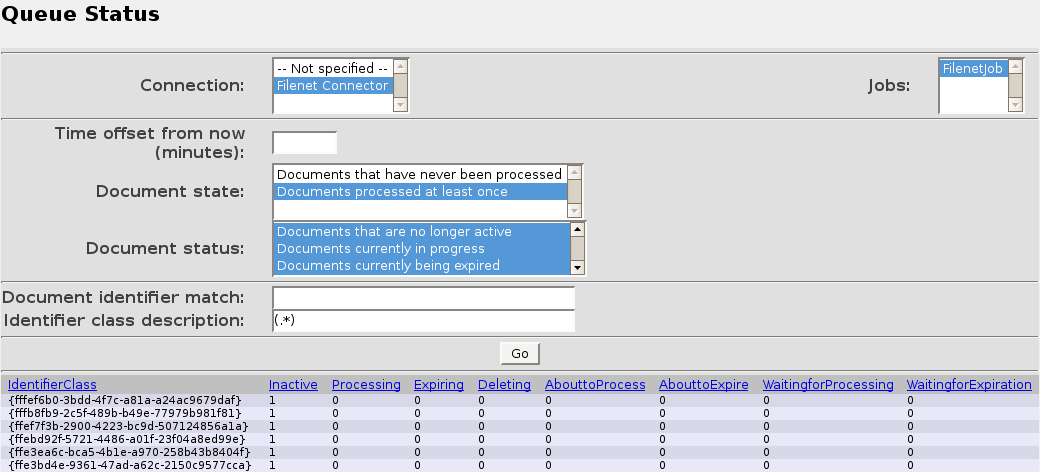
\includegraphics[width=300pt]{fln-queue-report}

This form offers the same fields as the Document Status report with
one addition, the \textbf{Identifier class description}, which allows
you to group results based on a regular expression. In this case, the
identifier class description is just \texttt{(.*)}, so each document
is shown individually as a group of one. If the regular expression
\texttt{(\^{}\{A)} was used, all documents whose identifiers began with
``A'' would be grouped together. Documents whose identifier started
with any other hexidecimal number would be analyzed together in the
first row of the table.


\note{If you are not familiar with regular expressions,
there are a variety of tutorials available on the web,
including \url{http://gnosis.cx/publish/}\linebreak
\url{programming/regular_expressions.html} and
\url{http://perldoc.}\linebreak\url{perl.org/perlrequick.html}. If you
still have difficulty with these settings, please contact Customer Support
(see page \pageref{SupportContact}).}


\subsection{History Reports}

The four types of history report are:

\begin{itemize}

\item Simple History, which lets you list an ordered set of log events
based on chosen criteria

\item Maximum Activity, which lets you see the period of time in
which a certain event happened most often

\item Maximum Bandwith, which lets you see the period of time in
which the most bandwidth was used 

\item Result Histogram, which provides log information that would be
appropriate for constructing a histogram or other diagram

\end{itemize}

Each of these reports allows you to specify a connection, one or more
activities, a start time, an end time, an entity match, and a result code
match.  Some also allow you to specify an identifier class description
and a sliding window size. This section will show sample results for
each type of report and an explanation of the fields selected.

\subsubsection{Simple History}

This report was generated by selecting ``Filenet Connector,'' 
clicking Continue, selecting ``document ingest,'' and clicking Go.

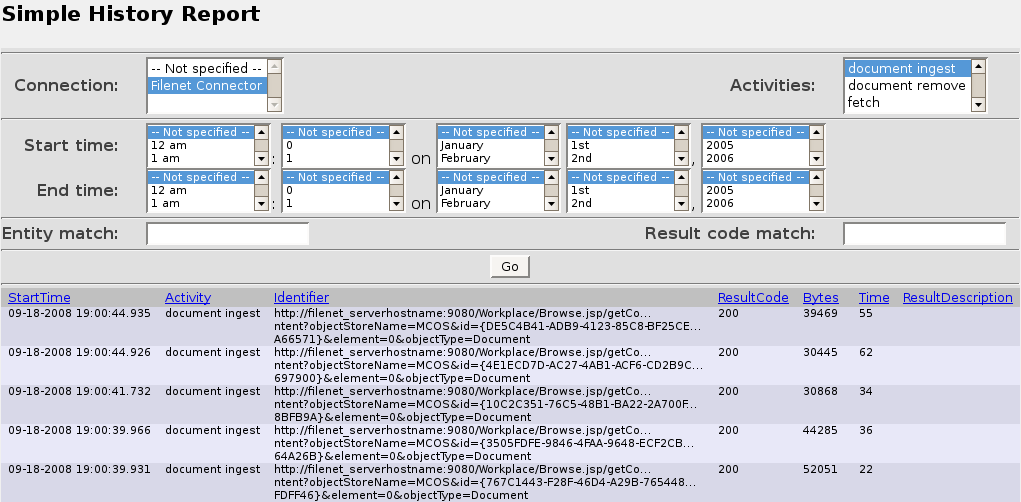
\includegraphics[width=300pt]{fln-simple-history-report}

\begin{itemize}

\item \textbf{Connection:} The repository connection from which to generate
a report.

\item \textbf{Activities}: What crawler activities you would like to
see.  Your options are document ingest, document remove, fetch, job
abort, job continue, job end, job start, and job wait.

\item \textbf{Start time}: The earliest time in the crawler logs to be
considered for this query.  Choose ``Not specified'' for any field to
start at the beginning of the crawler's logs.

\item \textbf{End time:} The latest time in the crawler logs to be
considered for this query. Choose ``Not specified'' for any field 
to end at the current time.

\item \textbf{Entity match:} A regular expression to limit the
Identifier field. In history reports, the document identifiers are
retrieval URLs, with the only unique portion being the document's
Filenet version GUID, described on page \pageref{docid}.

\item \textbf{Result code match:} A regular expression to limit the
ResultCode field.

\end{itemize}

You can sort the history report by any of the returned fields; to do so,
click the field names.

\subsubsection{Maximum Activity}

This report was generated by selecting ``Filenet Connector,'' clicking
Continue, selecting ``document ingest,'' changing the
Identifier class description, and clicking Go.

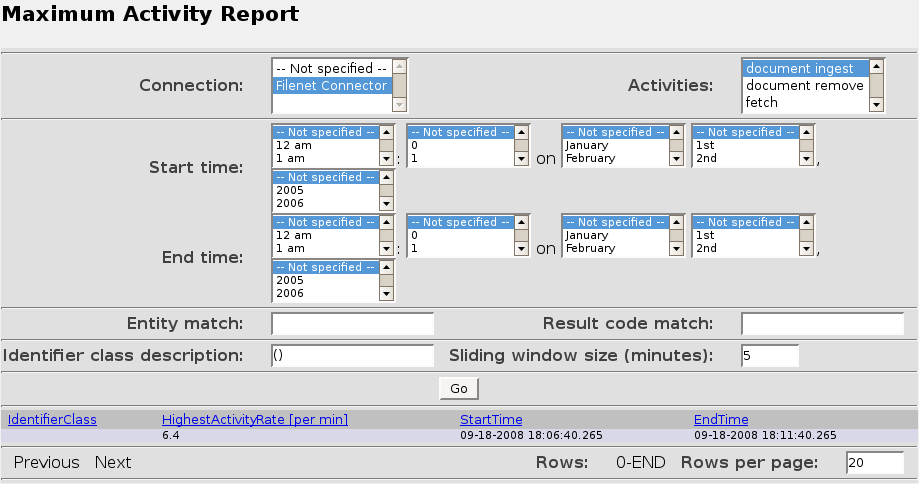
\includegraphics[width=300pt]{fln-maximum-activity-report}

This form offers two more fields than the previous form:

\begin{itemize}

\item \textbf{Identifier class description:} A regular expression that
determines how to group identifiers together. If this were set to
\texttt{(.*)}, there would be no grouping, and so there would be only
one ingestion event per document. The setting in the example,
\texttt{()}, groups all documents together.

\item \textbf{Sliding window size}: The search interval in minutes.

\end{itemize}

The report returned will have only one result per group with one or more
documents in it, if there is a clear highest activity rate, or a list of
all the results tied for highest activity rate if there are more than one.

\subsubsection{Maximum Bandwidth}

This report was generated by selecting ``Filenet Connector,'' clicking
Continue, selecting ``document ingest,'' changing the Identifier class
description, and clicking Go.

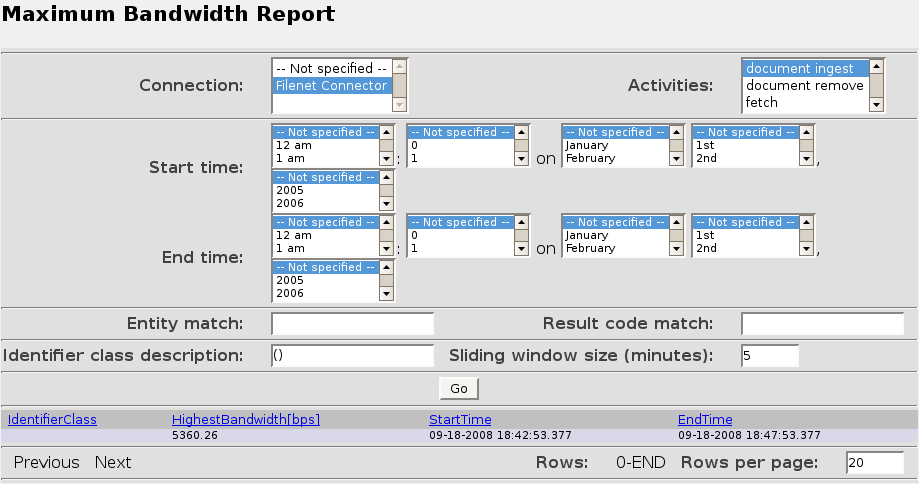
\includegraphics[width=300pt]{fln-maximum-bandwidth-report}

This form offers the same fields as the maximum activity form, and
returns similar results; instead of tracking events per time window,
it tracks the window with the highest average bandwith usage, measured
in bytes per second. Again, the identifier class description has been
changed to a regular expression that will match all identifiers (and
thus in this case all documents).

\subsubsection{Result Histogram}

This report was generated by selecting ``Filenet Connector,'' clicking
Continue, selecting ``document ingest,'' altering the identifier class
description to group documents based on their file path, and clicking
Go.

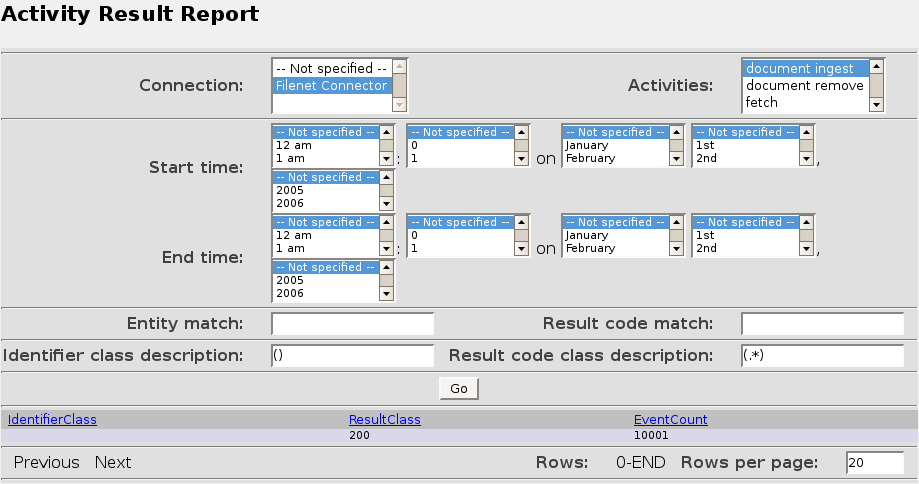
\includegraphics[width=300pt]{fln-activity-result-report}

This form adds one new field:

\begin{itemize}

\item \textbf{Result code class description:} A regular expression that
determines how to group result classes together; like Identifier class
descriptions but for result classes.

\end{itemize}

This report does not produce an actual histogram, but provides data that
could be used to generate histograms.  

\end{changemargin}
